\section*{Question 1.2 - Sieve of Eratosthenes - MPI (Multi-Machine)}

In this question we were asked to rewrite our earlier implementation of the 
Sieve of Eratosthenes using MPI, while utilizing `MPI\_send` and `MPI\_Recv`. 
Once complete we were then asked to run the code on three server and note the 
speed-up/slow-down when compared to previous implementations.

\subsection*{Results}

\begin{figure}
    \centering
    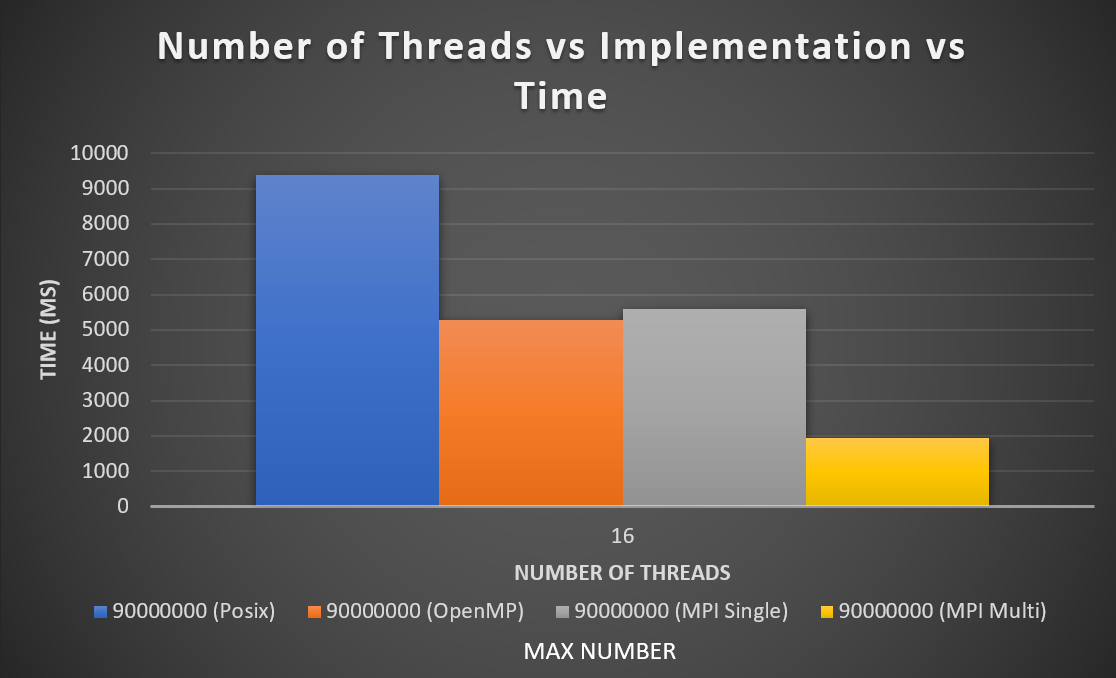
\includegraphics[width=\linewidth]{Figures/mpi_MULTI.png}
    \caption{Sieve of Eratosthenes with max number $9\times10^7$ on different
    implementations.}
    \label{fig:sievemulti}
\end{figure}

As seen in figure \ref{fig:sievemulti}, running the MPI implementation on multi-machines far 
outstripped our initial PThread version and OpenMP implementations.
This makes sense as we are now exploiting 3x the amount of cores we previously had.
Interestingly even though we now utilized 3x the amount of cores, we only saw a 
70\% improvement in terms of speed. This can be attributed to a number of factors:

\begin{itemize}
    \item Network Traffic and Latency
    \item Overhead the MPI adds when running on multiple-machines
    \item Time spent sending and receiving from the different machines
    \item The code which is still being run serially in the application
\end{itemize}